%{{第七十回}}{第七十回}}

\chapter{林黛玉重建桃花社\hspace{.5em}史湘云偶填柳絮词}

{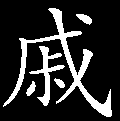
\includegraphics[width=3mm]{../Images/00005}\kaishu 空将佛事图相报,已触飘风散艳花。一片精神传好句,题成谶语任吁嗟!}

话说贾琏自在梨香院伴宿七日夜,天天僧道不断做佛事。贾母唤了他去,吩咐不许送往家庙中。贾琏无法,只得又和时觉说了,就在尤三姐之上点了一个穴,破土埋葬。那日送殡,只不过族中人与王信夫妇、尤氏婆媳而已。凤姐一应不管,只凭他自去办理。

因又年近岁逼,诸务猬集不算外,又有林之孝开了一个人名单子来,共有八个二十五岁的单身小厮应该娶妻成房,等里面有该放的丫头们好求指配。凤姐看了,先来问贾母和王夫人。大家商议,虽有几个应该发配的,奈各人皆有原故:第一个鸳鸯发誓不去。自那日之后,一向未和宝玉说话,也不盛妆浓饰。众人见他志坚,也不好相强。第二个琥珀,又有病,这次不能了。彩云因近日和贾环分崩,也染了无医之症。只有凤姐儿和李纨房中粗使的大丫鬟出去了,其馀年纪未足。令他们外头自娶去了。

原来这一向因凤姐病了,李纨探春料理家务不得闲暇,接着过年过节,出来许多杂事,竟将诗社搁起。如今仲春天气,虽得了工夫,争奈宝玉因冷遁了柳湘莲,剑刎了尤小妹,金逝了尤二姐,气病了柳五儿,连连接接,闲愁胡恨,一重不了一重添。弄得情色若痴,语言常乱,似染怔忡之疾。慌的袭人等又不敢回贾母,只百般逗他顽笑。

这日清晨方醒,只听外间房内咭咭呱呱笑声不断。袭人因笑说:“你快出去解救,晴雯和麝月两个人按住温都里那膈肢呢。”宝玉听了,忙披上灰鼠袄子出来一瞧,只见他三人被褥尚未叠起,大衣也未穿。那晴雯只穿葱绿院绸小袄,红小衣红睡鞋,披着头发,骑在雄奴身上。麝月是红绫抹胸,披着一身旧衣,在那里抓雄奴的肋肢。雄奴却仰在炕上,穿着撒花紧身儿,红裤绿袜,两脚乱蹬,笑的喘不过气来。宝玉忙上前笑说:“两个大的欺负一个小的,等我助力。”说着,也上床来膈肢晴雯。晴雯触痒,笑的忙丢下雄奴,和宝玉对抓。雄奴趁势又将晴雯按倒,向他肋下抓动。袭人笑说:“仔细冻着了。”看他四人裹在一处倒好笑。

忽有李纨打发碧月来说:“昨儿晚上奶奶在这里把块手帕子忘了,不知可在这里?”小燕说:“有,有,有,我在地下拾了起来,不知是那一位的,才洗了出来晾着,还未干呢。”碧月见他四人乱滚,因笑道:“倒是这里热闹,大清早起就咭咭呱呱的顽到一处。”宝玉笑道:“你们那里人也不少,怎么不顽?”碧月道:“我们奶奶不顽,把两个姨娘和琴姑娘也宾住了。如今琴姑娘又跟了老太太前头去了,更寂寞了。两个姨娘今年过了,到明年冬天都去了,又更寂寞呢。你瞧宝姑娘那里,出去了一个香菱,就冷清了多少,把个云姑娘落了单。”

正说着,只见湘云又打发了翠缕来说:“请二爷快出去瞧好诗。”宝玉听了,忙问:“那里的好诗?”翠缕笑道:“姑娘们都在沁芳亭上,你去了便知。”宝玉听了,忙梳洗了出来,果见黛玉、宝钗、湘云、宝琴、探春都在那里,手里拿着一篇诗看。见他来时,都笑说:“这会子还不起来,咱们的诗社散了一年,也没有人作兴。如今正是初春时节,万物更新,正该鼓舞另立起来才好。”湘云笑道:“一起诗社时是秋天,就不应发达。如今恰好万物逢春,皆主生盛。况这首桃花诗又好,就把海棠社改作桃花社。”{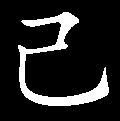
\includegraphics[width=3mm]{../Images/00003}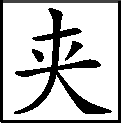
\includegraphics[width=3mm]{../Images/00012}\footnotesize \kaishu 起时是后有名,此是先有名。}宝玉听着,点头说:“很好。”且忙着要诗看。众人都又说:“咱们此时就访稻香老农去,大家议定好起的。”说着,一齐起来,都往稻香村来。宝玉一壁走,一壁看那纸上写着《桃花行》一篇,曰:

桃花帘外东风软,桃花帘内晨妆懒。

帘外桃花帘内人,人与桃花隔不远。

东风有意揭帘栊,花欲窥人帘不卷。

桃花帘外开仍旧,帘中人比桃花瘦。

花解怜人花也愁,隔帘消息风吹透。

风透湘帘花满庭,庭前春色倍伤情。

闲苔院落门空掩,斜日栏杆人自凭。

凭栏人向东风泣,茜裙偷傍桃花立。

桃花桃叶乱纷纷,花绽新红叶凝碧。

雾裹烟封一万株,烘楼照壁红模糊。

天机烧破鸳鸯锦,春酣欲醒移珊枕。

侍女金盆进水来,香泉影蘸胭脂冷。

胭脂鲜艳何相类,花之颜色人之泪;

若将人泪比桃花,泪自长流花自媚。

泪眼观花泪易干,泪干春尽花憔悴。

憔悴花遮憔悴人,花飞人倦易黄昏。

一声杜宇春归尽,寂寞帘栊空月痕!

宝玉看了并不称赞,却滚下泪来。便知出自黛玉,因此落下泪来,又怕众人看见,又忙自己擦了。因问:“你们怎么得来?”宝琴笑道:“你猜是谁做的?”宝玉笑道:“自然是潇湘子稿。”宝琴笑道:“现是我作的呢。”宝玉笑道:“我不信。这声调口气,迥乎不像蘅芜之体,所以不信。”宝钗笑道:“所以你不通。难道杜工部首首只作‘丛菊两开他日泪’之句不成!一般的也有‘红绽雨肥梅’、‘水荇牵风翠带长’之媚语。”宝玉笑道:“固然如此说。但我知道姐姐断不许妹妹有此伤悼语句,妹妹虽有此才,是断不肯作的。比不得林妹妹曾经离丧,作此哀音。”众人听说,都笑了。

已至稻香村中,将诗与李纨看了,自不必说称赏不已。说起诗社,大家议定:明日乃三月初二日,就起社,便改“海棠社”为“桃花社”,林黛玉就为社主。明日饭后,齐集潇湘馆。因又大家拟题。黛玉便说:“大家就要桃花诗一百韵。”宝钗道:“使不得。从来桃花诗最多,纵作了必落套,比不得你这一首古风。须得再拟。”正说着,人回:“舅太太来了。姑娘出去请安。”因此大家都往前头来见王子腾的夫人,陪着说话。吃饭毕,又陪入园中来,各处游顽一遍。至晚饭后掌灯方去。

次日乃是探春的寿日,元春早打发了两个小太监送了几件玩器。合家皆有寿仪,自不必说。饭后,探春换了礼服,各处去行礼。黛玉笑向众人道:“我这一社开的又不巧了,偏忘了这两日是他的生日。虽不摆酒唱戏的,少不得都要陪他在老太太、太太跟前顽笑一日,如何能得闲空儿。”因此改至初五。

这日众姊妹皆在房中侍早膳毕,便有贾政书信到了。宝玉请安,将请贾母的安禀拆开念与贾母听,上面不过是请安的话,说六月中准进京等语。其馀家信事务之帖,自有贾琏和王夫人开读。众人听说六七月回京,都喜之不尽。偏生近日王子腾之女许与保宁侯之子为妻,择日于五月初十日过门,凤姐儿又忙着张罗,常三五日不在家。这日王子腾的夫人又来接凤姐儿,一并请众甥男甥女闲乐一日。贾母和王夫人命宝玉、探春、林黛玉、宝钗四人同凤姐去。众人不敢违拗,只得回房去另妆饰了起来。五人作辞,去了一日,掌灯方回。宝玉进入怡红院,歇了半刻,袭人便乘机见景劝他收一收心,闲时把书理一理预备着。宝玉屈指算一算说:“还早呢。”袭人道:“书是第一件,字是第二件。到那时你纵有了书,你的字写的在那里呢?”宝玉笑道:“我时常也有写的好些,难道都没收着?”袭人道:“何曾没收着。你昨儿不在家,我就拿出来,共总数了一数,才有五六十篇。这三四年的工夫,难道只有这几张字不成。依我说,从明日起,把别的心全收了起来,天天快临几张字补上。虽不能按日都有,也要大概看得过去。”宝玉听了,忙的自己又亲检了一遍,实在搪塞不去,便说:“明日为始,一天写一百字才好。”说话时大家安下。至次日起来梳洗了,便在窗下研墨,恭楷临帖。贾母因不见他,只当病了,忙使人来问。宝玉方去请安,便说写字之故,先将早起清晨的工夫尽了出来,再作别的,因此出来迟了。贾母听了,便十分欢喜,吩咐他:“以后只管写字念书,不用出来也使得。你去回你太太知道。”宝玉听说,便往王夫人房中来说明。王夫人便说:“临阵磨枪,也不中用。有这会子着急,天天写写念念,有多少完不了的。这一赶,又赶出病来才罢。”宝玉回说不妨事。这里贾母也说怕急出病来。探春宝钗等都笑说:“老太太不用急。书虽替他不得,字却替得的。我们每人每日临一篇给他,搪塞过这一步就完了。一则老爷到家不生气,二则他也急不出病来。”贾母听说,喜之不尽。

原来林黛玉闻得贾政回家,必问宝玉的功课,宝玉肯分心,恐临期吃了亏。因此自己只装作不耐烦,把诗社便不起,也不以外事去勾引他。探春宝钗二人每日也临一篇楷书字与宝玉,宝玉自己每日也加工,或写二百三百不拘。至三月下旬,便将字又集凑出许多来。这日正算,再得五十篇,也就混的过了。谁知紫鹃走来,送了一卷东西与宝玉,拆开看时,却是一色老油竹纸上临的钟王蝇头小楷,字迹且与自己十分相似。喜的宝玉和紫鹃作了一个揖,又亲自来道谢。史湘云宝琴二人亦皆临了几篇相送。凑成虽不足功课,亦足搪塞了。宝玉放了心,于是将所应读之书,又温理过几遍,正是天天用功。可巧近海一带海啸,又遭蹋了几处生民。地方官题本奏闻,奉旨就着贾政顺路查看赈济回来。如此算去,至冬底方回。宝玉听了,便把书字又搁过一边,仍是照旧游荡。

时值暮春之际,史湘云无聊,因见柳花飘舞,便偶成一小令,调寄《如梦令》,其词曰:

岂是绣绒残吐,卷起半帘香雾,纤手自拈来,空使鹃啼燕妒。且住,且住!莫使春光别去。

自己作了,心中得意,便用一条纸儿写好,与宝钗看了,又来找黛玉。黛玉看毕,笑道:“好,也新鲜有趣。我却不能。”湘云笑道:“咱们这几社总没有填词。你明日何不起社填词,改个样儿,岂不新鲜些。”黛玉听了,偶然兴动,便说:“这话说的极是。我如今便请他们去。”说着,一面吩咐预备了几色果点之类,一面就打发人分头去请众人。这里他二人便拟了柳絮之题,又限出几个调来,写了绾在壁上。

众人来看时,以柳絮为题,限各色小调。又都看了史湘云的,称赏了一回。宝玉笑道:“这词上我们平常,少不得也要胡诌起来。”于是大家拈阄,宝钗便拈得了《临江仙》,宝琴拈得《西江月》,探春拈得了《南柯子》,黛玉拈得了《唐多令》,宝玉拈得了《蝶恋花》。紫鹃炷了一支梦甜香,{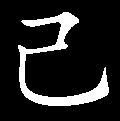
\includegraphics[width=3mm]{../Images/00003}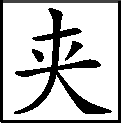
\includegraphics[width=3mm]{../Images/00012}\footnotesize \kaishu 重建,故又写香。}大家思索起来。一时黛玉有了,写完。接着宝琴宝钗都有了。他三人写完,互相看时,宝钗便笑道:“我先瞧完了你们的,再看我的。”探春笑道:“嗳呀,今儿这香怎么这样快,已剩了三分了。我才有了半首。”因又问宝玉可有了。宝玉虽作了些,只是自己嫌不好,又都抹了,要另作,回头看香,已将烬了。李纨笑道:“这算输了。蕉丫头的半首且写出来。”探春听说,忙写了出来。众人看时,{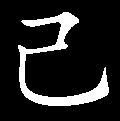
\includegraphics[width=3mm]{../Images/00003}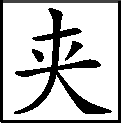
\includegraphics[width=3mm]{../Images/00012}\footnotesize \kaishu 却是先看没作完的,总是又变一格也。}上面却只半首《南柯子》,写道是:

空挂纤纤缕,徒垂络络丝,也难绾系也难羁,一任东西南北各分离。

李纨笑道:“这也却好作,何不续上?”宝玉见香没了,情愿认负,不肯勉强塞责,将笔搁下,来瞧这半首。见没完时,反倒动了兴开了机,乃提笔续道是:

落去君休惜,飞来我自知。莺愁蝶倦晚芳时,纵是明春再见,隔年期!

众人笑道:“正经你份内的又不能,这却偏有了。纵然好,也不算得。”说着,看黛玉的《唐多令》:

粉堕百花州,香残燕子楼。一团团逐对成球。飘泊亦如人命薄,空缱绻,说风流。  草木也知愁,韶华竟白头!叹今生谁舍谁收?嫁与东风春不管,凭尔去,忍淹留。

众人看了,俱点头感叹,说:“太作悲了,好是固然好的。”因又看宝琴的是《西江月》:

汉苑零星有限,隋堤点缀无穷。三春事业付东风,明月梅花一梦。  几处落红庭院,谁家香雪帘栊?江南江北一般同,偏是离人恨重!

众人都笑说:“到底是他的声调壮。‘几处’‘谁家’两句最妙。”宝钗笑道:“终不免过于丧败。我想,柳絮原是一件轻薄无根无绊的东西,然依我的主意,偏要把他说好了,才不落套。所以我诌了一首来,未必合你们的意思。”众人笑道:“不要太谦。我们且赏鉴,自然是好的。”因看这一首,《临江仙》道是:

白玉堂前春解舞,东风卷得均匀。

湘云先笑道:“好一个‘东风卷得均匀’!这一句就出人之上了。”又看底下道:

蜂团蝶阵乱纷纷。几曾随逝水,岂必委芳尘。  万缕千丝终不改,任他随聚随分。{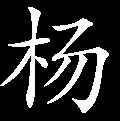
\includegraphics[width=3mm]{../Images/00008}\footnotesize \kaishu 人事无常,原不必戚戚也。}韶华休笑本无根,好风频借力,送我上青云!

众人拍案叫绝,都说:“果然翻得好。气力自然,是这首为尊;缠绵悲戚,让潇湘妃子;情致妩媚,却是枕霞;小薛与蕉客今日落第,要受罚的。”宝琴笑道:“我们自然受罚,但不知付白卷子的又怎么罚?”李纨道:“不要忙,这定要重重罚他。下次为例。”

一语未了,只听窗外竹子上一声响,恰似窗屉子倒了一般,众人唬了一跳。丫鬟们出去瞧时,帘外丫鬟嚷道:“一个大蝴蝶风筝挂在竹梢上了。”众丫鬟笑道:“好一个齐整风筝!不知是谁家放断了绳,拿下他来。”宝玉等听了,也都出来看时,宝玉笑道:“我认得这风筝。这是大老爷那院里娇红姑娘放的,拿下来给他送过去罢。”紫鹃笑道:“难道天下没有一样的风筝,单他有这个不成?我不管,我且拿起来。”探春道:“紫鹃也学小气了。你们一般的也有,这会子拾人走了的,也不怕忌讳。”黛玉笑道:“可是呢,知道是谁放晦气的,快掉出去罢。把咱们的拿出来,咱们也放晦气。”紫鹃听了,赶着命小丫头们将这风筝送出与园门上值日的婆子去了,倘有人来找,好与他们去的。

这里小丫头们听见放风筝,巴不得七手八脚都忙着拿出个美人风筝来。也有搬高凳去的,也有捆剪子股的,也有拨籰子的。宝钗等都立在院门前,命丫头们在院外敞地下放去。宝琴笑道:“你这个不大好看,不如三姐姐的那一个软翅子大凤凰好。”宝钗笑道:“果然。”因回头向翠墨笑道:“你把你们的拿来也放放。”翠墨笑嘻嘻的果然也取去了。宝玉又兴头起来,也打发个小丫头子家去,说:“把昨儿赖大娘送我的那个大鱼取来。”小丫头子去了半天,空手回来,笑道:“晴姑娘昨儿放走了。”宝玉道:“我还没放一遭儿呢。”探春笑道:“横竖是给你放晦气罢了。”宝玉道:“也罢。再把那个大螃蟹拿来罢。”丫头去了,同了几个人扛了一个美人并籰子来,说道:“袭姑娘说,昨儿把螃蟹给了三爷了。这一个是林大娘才送来的,放这一个罢。”宝玉细看了一回,只见这美人做的十分精致。心中欢喜,便命叫放起来。此时探春的也取了来,翠墨带着几个小丫头子们在那边山坡上已放了起来。宝琴也命人将自己的一个大红蝙蝠也取来。宝钗也高兴,也取了一个来,却是一连七个大雁的,都放起来。独有宝玉的美人放不起去。宝玉说丫头们不会放,自己放了半天,只起房高便落下来了。急的宝玉头上出汗,众人又笑。宝玉恨的掷在地下,指着风筝道:“若不是个美人,我一顿脚跺个稀烂。”黛玉笑道:“那是顶线不好,拿出去另使人打了顶线就好了。”宝玉一面使人拿去打顶线,一面又取一个来放。大家都仰面而看,天上这几个风筝都起在半空中去了。

一时丫鬟们又拿了许多各式各样的送饭的来,顽了一回。紫鹃笑道:“这一回的劲大,姑娘来放罢。”黛玉听说,用手帕垫着手,顿了一顿,果然风紧力大,接过籰子来,随着风筝的势将籰子一松,只听一阵豁刺刺响,登时籰子线尽。黛玉因让众人来放。众人都笑道:“各人都有,你先请罢。”黛玉笑道:“这一放虽有趣,只是不忍。”李纨道:“放风筝图的是这一乐,所以又说放晦气,你更该多放些,把你这病根儿都带了去就好了。”紫鹃笑道:“我们姑娘越发小气了。那一年不放几个子,今忽然又心疼了。姑娘不放,等我放。”说着便向雪雁手中接过一把西洋小银剪子来,齐籰子根下寸丝不留,“咯登”一声铰断,笑道:“这一去把病根儿可都带了去了。”那风筝飘飘摇摇,只管往后退了去,一时只有鸡蛋大小,展眼只剩了一点黑星,再展眼便不见了。众人皆仰面睃眼说:“有趣,有趣。”宝玉道:“可惜不知落在那里去了。若落在有人烟处,被小孩子得了还好,若落在荒郊野外无人烟处,我替他寂寞。想起来把我这个放去,教他两个作伴儿罢。”于是也用剪子剪断,照先放去。

探春正要剪自己的凤凰,见天上也有一个凤凰,因道:“这也不知是谁家的。”众人皆笑说:“且别剪你的,看他倒像要来绞的样儿。”说着,只见那凤凰渐逼近来,遂与这凤凰绞在一处。众人方要往下收线,那一家也要收线,正不开交,又见一个门扇大的玲珑喜字带响鞭,在半天如钟鸣一般,也逼近来。众人笑道:“这一个也来绞了。且别收,让他三个绞在一处倒有趣呢。”说着,那喜字果然与这两个凤凰绞在一处。三下齐收乱顿,谁知线都断了,那三个风筝飘飘摇摇都去了。众人拍手哄然一笑,说:“倒有趣,可不知那喜字是谁家的,忒促狭了些。”黛玉说:“我的风筝也放去了,我也乏了,我也要歇歇去了。”宝钗说:“且等我们放了去,大家好散。”说着,看姊妹都放去了,大家方散。黛玉回房歪着养乏。要知端的,下回便见。

{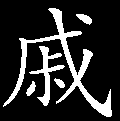
\includegraphics[width=3mm]{../Images/00005}\kaishu 总评:文与雪天联诗篇一样机轴,两样笔墨。前文以联句起,以灯谜结,以作画为中间横风吹断,此文以填词起,以风筝结,以写字为中间横风吹断,是一样机轴;前文叙联句详,此文叙填词略,是两样笔墨,前文之叙作画略,此文叙写字详,是两样笔墨。前文叙灯谜,叙猜灯谜,此文叙风筝,叙放风筝,是一样机轴;前文叙七律在联句后,此文叙古歌在填词前,是两样笔墨。前文叙黛玉替宝玉写诗,此文叙宝玉替探春续词,是一样机轴,前文赋诗后有一首诗,此文填词前有一首词,是两样笔墨。噫!参伍其变,错综其数,此固难为粗心者道也!}
